\chapter{Automatic Pattern Detection with \ql{}}\label{ap:ql}



\textbf{Source Code Analysis.}
We have implemented our study using the \ql{} query language:
% ``a declarative, object-oriented logic programming language for querying complex, potentially recursive data structures encoded in a relational data model''~\cite{avgustinov_ql:_2016}.
\ql{} allows us to analyze programs at the source code level by abstracting the code sources into a relational data model.
Besides providing structural data for programs, \ie{}, ASTs, \ql{} has the ability to query static types and data-flow analysis.
To run our \ql{} queries, we have used the service provided by Semmle.\footnote{\url{https://lgtm.com/}} 


The typecase pattern consists of testing the runtime type of a variable against several related types.
Based on rule taken from:
It was taken from a \lgtm{} rule\footnote{\url{https://lgtm.com/rules/910065/}}.

% \begin{pattern}{Deserialization}
% Used to deserialize an object.
    
% \instances
    
% https://lgtm.com/projects/g/mockito/mockito/snapshot/da68900466a17e21fef3e27690f4cef4b5c240ea/files/src/test/java/org/mockitoutil/SimpleSerializationUtil.java?sort=name&dir=ASC&mode=heatmap&showExcluded=false#L29
    
% \begin{lstlisting}[style=java,caption={Instance of the \pname{} pattern  (\url{http://bit.ly/2KOpj3A}) }]
%     Object readObject = new ObjectInputStream(unserialize).readObject();
%     assertNotNull(readObject);
%     return type.cast(readObject);
%     \end{lstlisting}
    
% \detection
    
% \begin{lstlisting}[style=ql]
% DeserializationCastPattern() {
%     this instanceof ReadObjectCastTag
% }
% \end{lstlisting}
    
% \end{pattern}
    
ExceptionSoftening
We can throw CheckedExceptions even on methods that don't declare them (via Exception softening).
    
    








\section{Is the cast operator used?}

\label{sec:stats}

% To answer \ref{enum:rq1} we want to know how many cast instances are used in a given project.
To this end, we gather the following statistics using \ql{}.
We show them here to give an estimation of the size of the code base being analized.

% \begin{center}
% \begin{tabular}{lr}
% 	Description & Value\\
% 	\hline
% 	Number of Projects & \nproject{} \\
% 	Number of LOC & \nloc{} \\
% 	Number of Methods & \nmethod{} \\
% 	Number of Methods \emph{w/}Cast & \nmethodwithcast{} \\
% 	Number of Exprs & \nexpr{} \\
% 	Number of Casts & \nCastExpr{} \\
% \end{tabular}
% \end{center}

The \emph{Number of Methods} and \emph{Number of Methods w/Cast} values includes only methods with a body, \ie{}, not abstract, nor native.
The \emph{Number of Exprs} value show how many expressions there are in the ASTs of all source code analyzed.
Finally, the \emph{Number of Casts} value indicates how many cast expressions (subtype of \code{Expr} as defined by \ql{}) were found.

For our study, we are interested in both upcasts and downcasts.
This is why we want to exclude any primitive conversion in our study.
The \emph{Number of Casts} value shown above include only reference conversions.
Primitive conversions are always safe (in terms of throwing \code{ClassCastException}.
A primitive conversion happens when both the type of the expression to be casted to and the type to cast to are primitive types.
Note that with this definition, we include in our study \emph{boxed} types.
Since boxed types are reference types (and therefore not necessarily safe)
we want to include them for our analysis.

We want to know how many cast instances there are across projects.
Thus, we have computed the ratio between methods containing at least a cast over total number of methods --- with implementation --- in a given project.
The following chart shows this ratio for all analyzed projects:

% 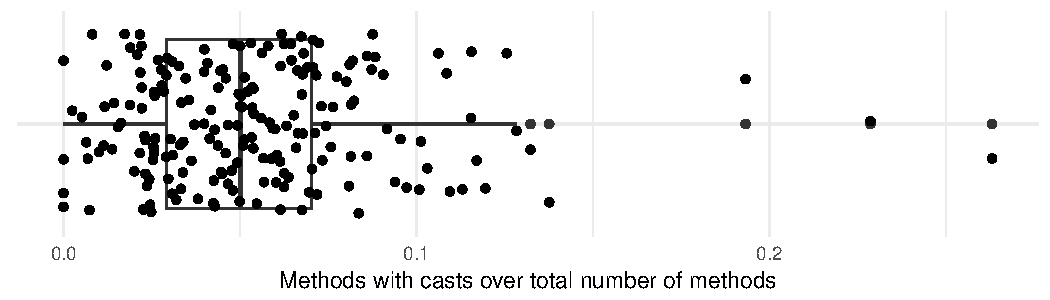
\includegraphics[width=\columnwidth]{../analysis/stats-methodwcastXproject.pdf}

All projects have less than $10\%$ of methods with at least a cast.
% Overall, around a~$\castpercentage{}$ of methods contain at least one cast operation. 
This means there is a low density of casts.
Given the fact that generics were introduced \java{} 5, this can explain this low density.

Nevertheless, casts are still used.
% We want to understand why there are casts instances (\ref{enum:rq2}) and how often the use cases that leads to casts are used (\ref{enum:rq3}).
The following sections give an answer to these questions.

The query to gather this statistics is available online.\footnote{\url{https://gitlab.com/acuarica/java-cast-queries/blob/master/stats.ql}}
% The \R{} script to further analyze the query results is available online as well.\footnote{\url{https://gitlab.com/acuarica/java-cast-queries/blob/master/stats.r}}







\section{Finding Casts Usage Patterns}

\label{sec:methodology}

% To answer both research questions \ref{enum:rq2} and \ref{enum:rq3} we have used the \ql{} query language within the \lgtm{} service to look for cast instances.
As mentioned in section \ref{sec:stats}, \ql{} treats primitive conversions as casts.
Thus, a preliminary step is to exclude them as cast instances.
The following \ql{} query shows how to retrieve all relevant cast expressions:

% \begin{lstlisting}[style=ql,caption=\ql{} query to retrieve all relevant cast expressions.]
% import java
% from CastExpr ce where not (
% ce.getExpr().getType() instanceof PrimitiveType and
% ce.getTypeExpr().getType() instanceof PrimitiveType
% ) select ce
% \end{lstlisting}

Figure~\ref{fig:process} depicts our methodology.
We have used this initial result as a starting point for our analysis.
Afterwards, we select a random sample for manual inspection.
We manually inspected the mentioned casts trying to understand why and how they were used.

By manually inspecting several casts instances, we observe that certain characteristics appear often, \eg{}, a cast in a overridden method, or a cast guarded by an \code{instanceof}.
We then \emph{tag} cast instances based on these observations.
We implement a \ql{} predicate that detects them and proceed to refine our query with this new tag predicate.
The table of tags is presented in table~\ref{table:tags}.
After a new tag is added, the query is run again to iterate over the new results.

Whenever we observe that those tags do not appear randomly, we further inspect the source code to check that is indeed a pattern.
We have formalize the structure of each pattern as a \ql{} predicate based on those tags.
Similarly with tags, after a new pattern is added, the query is run again to inspect the casts without pattern.
To sum it up, our methodology iterates over the results until no patterns can be detected.
% These patterns are presented in the following section.
The final \ql{} query is available online.\footnote{\url{https://gitlab.com/acuarica/java-cast-queries/blob/master/casts.ql}}

\tikzstyle{decision} = [diamond, aspect=2, draw, fill=blue!20, 
    text width=6em, text badly centered, node distance=3cm, inner sep=0pt]
\tikzstyle{block} = [rectangle, draw, fill=blue!20, 
    text width=7em, text centered, rounded corners, minimum height=2em]
\tikzstyle{line} = [draw, -latex']
\tikzstyle{cloud} = [draw, ellipse,fill=red!20, node distance=3cm,
    minimum height=2em]

\begin{figure}[ht]
\centering
\begin{tikzpicture}[node distance = 1.3cm, auto]
    % Place nodes
    \node [block] (run) {Run Query};
    \node [cloud, left of=run] (tags) {Tags};
    \node [cloud, right of=run] (patterns) {Patterns};
    \node [block, below of=run] (inspect) {Inspect Casts without Pattern};
    \node [decision, below of=inspect, node distance=1.6cm] (tag) {New Tag?};
    \node [decision, below of=tag, node distance=1.8cm] (pattern) {New Pattern?};
    \node [block, left of=tag, node distance=3cm] (update-tags) {Update Tags};
    \node [block, right of=pattern, node distance=3cm] (update-pattern) {Update Patterns};
    % \node [decision, below of=evaluate] (decide) {is best candidate better?};
    \node [block, below of=pattern, node distance=1.5cm] (stop) {Stop};
    % Draw edges
    \path [line] (run) -- (inspect);
    % \path [line] (inspect) -- (evaluate);
    \path [line] (inspect) -- (tag);
    % \path [line] (inspect) -- (pattern);
    \path [line] (tag) -- node [near start] {yes} (update-tags);
    \path [line] (pattern) -- node [near start] {yes} (update-pattern);
    \path [line] (update-tags) -- (tags);
    \path [line] (update-pattern) -- (patterns);
    \path [line] (tag) -- node {no}(pattern);
    \path [line] (pattern) -- node {no}(stop);
    \path [line,dashed] (tags) -- (run);
    \path [line,dashed] (patterns) -- (run);
\end{tikzpicture}
\caption{Process to discover cast tags and patterns} \label{fig:process}
\end{figure}

\definecolor{header-color}{HTML}{D1D1D1}
\definecolor{alt-row-color}{HTML}{ECECEC}

% \newcommand{\hdr}{\rowcolor{header-color}}
% \newcommand{\alt}{\rowcolor{alt-row-color}}
% \newcommand{\row}{}
\begin{table*}[t!]
\centering
\caption{Cast tags used to discover cast patterns.}
\label{table:tags}
\end{table*}